
%------------------------------------------------------------------------------
\section{Preliminary concepts}
%------------------------------------------------------------------------------
\label{sec:disr_concepts}

\subsection{Basic Idea}
The main concept behind of the original SR approach is the
\emph{Segment}: a Segment is basically a path of consecutive node
and links. All segments start with a link attached to a node which
belongs to different segment, ending with a link also attached to a
node belonging to a different segment. A exception is the first
segment estabilished in the network, called \emph{starting segment} which is  a loop
beginning/ending on a particular node defined as bootstrap node.

The idea is to partition the network in a set of disjoint segments, and then
placing a turn restriction within each segment. It has been proved~\cite{mejia_ipdps06}
that such a set of turn prohibitions guarantees dealock freedom and
while preserving connectivity of the network.

Describing the execution phases of DiSR from a top level point-of-view
is basically similar to the classic SR approach. This can be useful to
give an initial idea of the approach, however, some essential
differences should be pointed out. First of all no centralized entity is
globally aware of what is going on: the status of the DiSR execution
is collectively distributed among the nodes; second, no defect map and/or
topology graph is available as input, thus, the topology has to be
discovered \emph{while} segments are created; finally, at the end of the
execution, no segment list is created: Each node is only aware of
belonging to some segment, ignoring the presence of other nodes
in the same segment and even the presence of other segments in the
network.

Roughly speaking, the execution of can be described as the execution
of the following phases:
\begin{itemize}
\item Injection of the DiSR process from upper layer to set a bootstrap
node
\item Bootstrap node broadcasting to create the first segment of the subnet
\item Parallel requests starting from assigned node to discover other segments
%\item Turn proibition in each confirmed segment
%\item Draining of remaining packet due timeouts
\end{itemize}

Once again, it should be pointed out that nowhere in the network there
is such a global vision of these exection phases. A more detailed
description of the exection model at each node is discussed in the
next section.

\subsection{Packets types Required}

The DiSR approach works with a distributed mechanism which is build
upon an exchange of small packets containing the following fields:
\begin{itemize}
\item{packet\_type}: encodes the meaning of the control message respect
to the whole DiSR process.
\item{seg\_ID}: the id of the segment associated to the DiSR control message
\item{src\_id}: the id of the node that initially originated the
packet
\end{itemize}

As regards packet\_type, we can have the following control packets:
\begin{itemize}
\item{\texttt{STARTING\_SEGMENT\_REQUEST}}: Injected by the bootstrap
node to when searching for the first segment. 
\item{\texttt{STARTING\_SEGMENT\_CONFIRM}}: used when estabilishing
the starting  segment. 
\item{\texttt{SEGMENT\_REQUEST}}: used to search candidates for a segment (not the
first)
\item{\texttt{SEGMENT\_CONFIRM}}: used to estabilish a segment. 
\item{\texttt{SEGMENT\_CANCEL}}: used to cancel the process of searching a segment along a
specific link.
\end{itemize}

A quantitative analysis of the resources needed to implement these
fields is presented in Section~\ref{sec:implementation} when
discussing the impact of the DiSR control logic and storage on
hardware implementation of the node.

\subsection{DiSR Data Structures}
\label{ssec:disr_dstruct}

We distinct between two different kind of data stored at each node:
\emph{Local Environment Data} (\emph{LED}) and \emph{Dynamic Behaviour
Status} (\emph{DBS}).

The \emph{LED} is like a snapshot of the DiSR algorithm at each node,
consisting in the following variables:

\begin{itemize}
\item{\emph{segID}}:a value used to specify the segment to which the
node has been assigned or is candidate for being assigned.
\item{\emph{visited}}: a boolean value. When \emph{true}
a \emph{segID} different from \texttt{NULL} specifies the segment 
to which the node has been assigned. 

% TODO: the following is true, but complicates things at this stage
%Note that a value different from \emph{NULL} does not
%necessarily mean the node has been assigned to some segment (e.g. when
%searching starting segment is set \emph{visited} by default even if not yet
%assigned to any segment). 

\item{\emph{tvisited}}: a boolean value. If \emph{true}, the node is
being considered as candidate for a segment, and the \emph{segID} value
specifies the segment id for which the node is candidate. 
\item{\emph{link\_visited[]}}: an array
of values representing information about attached links, that is, the
segID of the segment owning each link. When \texttt{NULL}, the corresponding link has not yet been
assigned.
%TDB: do we need to introduce some value for the
%“bridge” status ? (e.g. a node connecting the terminal node of a
%subnet with the starting one of another) 
\item{\emph{link\_tvisited[]}}: an array of
values representing information about attached links, that is, the \emph{segID} of
the segment for which the link is candidate. When \texttt{NULL}, the link is
currently not \emph{tvisited}.  
\end{itemize}
%\item{\emph{starting}}: boolean, \emph{true} if the node is a
%starting node from which the whole process was initiated.
%\end{itemize}

In addition to the \emph{LED} variables described above, further
information should be stored in order to capture the current dynamic
behaviour of the node. This is represented by \emph{DBS} variable,
which strictly depends on the \emph{LED} data and the events occurring
at the node. The \emph{DBS} can have the following values:

\begin{itemize}
\item{\emph{Free}}: a node that has  not been yet considered  by the DiSR algorithm.
The node is not marked as \emph{visited}/\emph{tvisited}.
\item{\emph{Bootstrap}}: a node which has been explicitly set as bootstrap node from
an upper layer via. 
% TODO: this and all the other details on the items below should be
% checked and moved elsewhere for a future long paper

%This is required because a
%\texttt{STARTING\_SEGMENT\_REQUEST} packet should be injected in order to start
%the whole process.
\item{\emph{ActiveSearching}}: a node from which a find process of new segments has
been started and not yet cancelled or confirmed. 
%This happens when all
%the following conditions are matched: the node is marked as \emph{visited},
%that is \emph{visited} = TRUE 
%TODO: \emph{segID} is set to some value reflecting
%the segment request sent there is a link that is being investigated by
%the node, that is a tvisited\_link marked with the same id of the node 
\item{\emph{Candidate}}: a node currently candidate for belonging to some segment
with id segid, not being itself the node from which the find process
was started. 

%The following conditions should be matched: \emph{tvisited} =
%true, with segID=X different from node's id.  Two links set as
%\emph{link\_tvisited} with id X. Let’s refer them as  links 'i' and 'j'. Then
%link\_tvisited[i] was set = X when the find process from an adjacent
%node reached the current node, while link\_tvisited[j] has been set to
%X when the node itself started to investigate its free links for the
%segment request with id X. Note that while investigating its attached
%links, if the find process fails along path 'j', the current node can
%investigate another free node 'k' if suitable.  
\item{\emph{CandidateStarting}}: same as above, but the node is currently being considered as candidate
for starting segment. 

%Two main differences: Can confirm
%\texttt{STARTING\_SEGMENT\_CONFIRM} with the same \emph{segID} when receiving a normal
%\texttt{SEGMENT\_REQUEST}: Overwrites its status setting it to \emph{Candidate} for the
%segID frees the links previously set as \emph{tvisited} during flooding
\item{\emph{Assigned}}: a node for which the segment has been determined.  The
segment \emph{segID} attribute value is set to some id X different from \texttt{NULL}.
%The \emph{visited} value is \emph{true} NOTE: an \emph{Assigned} state is a quick temporary
%state, since it becomes \emph{ActiveSearching} if a not (\emph{visited}/tvisited)
%link is suitable for searching new segments (see next\_visited
%procedure on paper) 
\end{itemize}


\subsection{Sketch of DiSR}

\begin{itemize}

\item{\textbf{Injecting bootstrap request}}: all nodes have a initial
\emph{DBS} status \emph{Free}, except for a
 node with status \emph{Bootstrap}, set by some signal from an
upper layer via. When starting, this bootstrap node sets itself as \emph{visited} and
changes its status to \emph{ActiveSearching}, injecting a
\texttt{STARTING\_SEGMENT\_REQUEST} across one of its free links. 

\item{\textbf{Flooding}}: Each node receiving a \texttt{STARTING\_SEGMENT\_REQUEST},
if not yet (\emph{visited}/\emph{tvisited}),  forwards it to its free links using a flooding mechanism.
Each of these links is then marked as \emph{tvisited} with the segment id
associated to the request. Note that a node that has already received a
\texttt{STARTING\_SEGMENT\_REQUEST} packet can simply ignore further packets
associated to the same request, having already contributed to the
flooding. 
%Note also that each of these packets has a max\_segment\_hops
%field to prevent packets from travelling undefinitively.  

\item{\textbf{Confirming the Starting Segment}}: when this \texttt{STARTING\_SEGMENT\_REQUEST} packet reaches
the starting node (from a different link, of course), the starting
segment is found. Then the starting node sends back a \texttt{STARTING\_SEGMENT\_CONFIRM}
packet with the same id along the link from which it received the
\texttt{STARTING\_SEGMENT\_REQUEST}. Each node do same by changing its own status
to \emph{Assigned}. So the confirmation packet is sent back from
node to node and the starting segment is created. 

Note: A node knows to be \emph{Candidate} due a
\texttt{STARTING\_SEGMENT\_REQUEST}.  Then, when receiving a simple
(not starting) \texttt{SEGMENT\_REQUEST} , it can simply cancel its
previous \emph{Candidate} status, since this second
request means that the starting segment has already been found. 

%What happens to nodes not receiving these segment request?
%they simply remain \emph{tvisited} and after a timeout reset their
%state as free. But they could also remain \emph{tvisited} for the
%starting segment, since this doesn’t affect their behaviour for future
%segment requests.  

%failure: TODO should we handle this case ? i.e.  marking as terminal ?

\item{\textbf{Injecting other request}}: Each node in the \emph{Assigned} status can initiate a search for a
segment, by sending a \texttt{SEGMENT\_REQUEST} across one of its free
links. Note that, since this is not the starting segment, in this case
the packet should not return back to the initiator, but just another visited
node
\item{\textbf{Setup of a segment}}: The find process is successfull
when an \emph{Assigned} node receives the \texttt{SEGMENT\_REQUEST} packet. Then, a \texttt{SEGMENT\_CONFIRM} is
sent back along the path that originated the request.  
\item{\textbf{Failing while searching a segment}}: a node received a \texttt{SEGMENT\_REQUEST} packet but
matched one of the following conditions: the node is free but has no
more suitable free links (can’t forward the \texttt{SEGMENT\_REQUEST}) the node
is \emph{tvisited} candidate for another find process the request packet
exceeded the max\_segment\_hops limit.  In all these cases the node
sends back a \texttt{SEGMENT\_CANCEL} along the proper link modifying its state
to free. Each of the subsequent nodes will forward this \texttt{SEGMENT\_CANCEL}
only if no more free links can be explored starting from them.
\end{itemize}


%\subsection{Intra-node vs Inter-node parallelism}
%In the processes described above, we assumed that each node in the
%READY\_SEARCHING state can start a find segment process by injecting a
%\texttt{SEGMENT\_REQUEST}. However, a more accurate decision when defining DiSR
%should be made in order to decide whether or not the node must
%actually perform this action. 
%The point above is is strictly related to the general question: which
%level of “parallelism” should we allow in DiSR ? The adopted approach
%is that, although the nature of DiSR itself is intrinsicly parallel,
%the use of parallelism makes things work in a more complex way. In
%other words, DiSR is parallel when needed, but it does not exploit
%parallelism as an “improving feature”. When not needed, things should
%be serialized. For example: when a node is “ready searching” could
%start several find segment process associated to the same segment, one
%for each free link. But serializing this by investigating the free
%links in order could be a simplest solution. We refer to this saying
%that we avoid intra-node parallelism.  Note that while intra-node
%parallelism can be avoided, trying to avoid inter-node parallelism
%could be more complex than allowing the parallelism itself. Imagine
%for example the effort of trying to coordinate nodes so that an unique
%finding node process is actually running in the whole subnet. Thus, in
%contrast to the intra-node parallelism, the inter-node parallelism is
%a structural property of the DiSR algorithm and should not be avoided.
%------------------------------------------------------------------------------

\section{Detailed Node behaviour Model}
\label{sec:execution_model}

The \emph{LED} variables at each node are are initially set so the node and
each of its links is set as free. The only node that makes exception
is the bootstrap node, initialized in the \emph{Bootstrap} status. All
the subsequent events happening at each node are the consequence of
its current dynamic status (DBS) and the packets received.

\begin{figure}
  \centering
    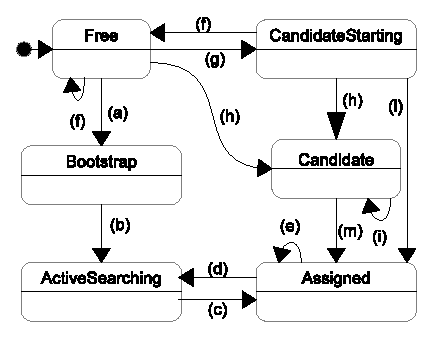
\includegraphics[width=0.30\textwidth]{pictures/state_machine.eps}
  \caption{DiSR node execution model}
  \label{fig:dna_tag}
\end{figure}

%TODO: add state machines

% TODO: fix, move elsewhere or delete
%Assumption: when discussing of visited/\emph{tvisited} nodes, we are assuming
%with an id corresponding to the same subnet. Nodes involved in other
%subnet processes can simply ignore these packets. (TBD: formalize more
%clearly in which cases inter-subnet packets must be ignored, probably
%this happens most of the times, but in some cases, e.g. when a
%terminal node is found, some kind of communication packets are needed
%in order to crearte the bridge between two subnets.) 

\subsection{Receiving a \texttt{STARTING\_SEGMENT\_REQUEST}}

The request for the first segment should be managed differently since
all nodes (except the starting one) must forward the packet using a
flooding mechanism. This is necessary since the request packet must
return the bootstrap node.
When a node receives a \texttt{STARTING\_SEGMENT\_REQUEST}, the
following cases can happen:

\begin{itemize}
\item The node is not candidate or assigned: it should set itself as
\emph{Candidate} and forward the packet along its free links, using
flooding.  
\item The node is \emph{Candidate} with the same
\emph{segID} and \emph{src\_id} is equal to node id: this means the
node was the initiator of the request, so a starting segment was found and
should be confirmed sending back a \texttt{STARTING\_SEGMENT\_CONFIRM}
packet.  
\item The node is \emph{Candidate}, with the same \emph{segID} of the
packet but \emph{src\_id} is different from node id: due
the flooding mechanism, another starting segment packet reached a node
which was previously marked as \emph{Candidate} from the same starting segment
search process. Since the node is candidate with the same id, it means
that it already accomplished in the task of propagating that kind
packets, thus can simply ignore the event thrashing the packet.  
%TBD: how the status should be changed ? depend on the flooding mechanism. Note
%that these links do not include the link from which the request was
%received.  
\item The node is \emph{Candidate}, with a different \emph{segID}: 
this simply means that the starting segment received is deprecated,
because the node has already accepted non-starting segment requests
originated from other \emph{Assigned} nodes.
\item The node is \emph{Assigned}, with a different \emph{segID}:
same as the previous case. 

% TODO: check and remove, the below is not true
%CHECK:  it is not the initiator of the starting segment request, but
%is already assigned to some segment!? assuming again we are discussing
%of nodes belonging to the same subnet, this should NOT happen, since
%the only visited node of the subnet should be the initial node from
%which the \texttt{STARTING\_SEGMENT\_REQUEST} originated. Note again that we are
%assuming that if the the node is visited or \emph{tvisited} with the id of
%another subnet can simply ignore the request.  The node is \emph{tvisited}
%but it is not the initiator of the request (different id): same as
%above, if we are assuming nodes of the same subnet, this should not
%happen. If the node is of another subnet, can simply ignore the event.

\end{itemize}

\subsection{Receiving a \texttt{SEGMENT\_REQUEST}}
When a node receives a \texttt{SEGMENT\_REQUEST}, the are the following cases:

\begin{itemize}
\item The node is \emph{Assigned}: a segment was
found and it should be confirmed sending back a \texttt{SEGMENT\_CONFIRM}
packet.  
\item The node is \emph{Candidate}: it should discard the packet sending
back a \texttt{SEGMENT\_CANCEL} 
\item The node is not \emph{Assigned} or \emph{Candidate} and has free
links: it marks itself as \emph{Candidate} and forwards the \texttt{SEGMENT\_REQUEST}
to one of its free links, according to some internal ordering
\end{itemize}

NOTE: the main difference between confirming a \texttt{STARTING\_SEGMENT\_REQUEST}
and confirming a \texttt{SEGMENT\_REQUEST} is that in the first case the node
itself is included in the segment , while in the second case the
receiving node does not belong to the segment found. 

%The motivation is
%that in the second case the node was already marked as \emph{visited} because
%of being assigned to some segment found before, while in the
%starting-segment case, by definition, the first segment of a subnet
%begins with the starting node, which is marked as \emph{visited} by the SR
%algorithm when searching for the first (starting) segment. Remember
%that the first segment of a subnet is a loop beginning with the
%starting node. 

\subsection{Receiving a \texttt{SEGMENT\_CONFIRM}}
When received, if the node status is \emph{Candidate} with a \emph{segID} corresponding to the one indicated in
the packet, the node learns to belong to the segment associated to the
id. Further, it should forward this packet to the link where the
original \texttt{SEGMENT\_REQUEST} packet came from, so that all candidate nodes
can learn the segment id they belong to.  \emph{LED} shoud be
updated: The state of the node changes from \emph{tvisited} to \emph{visited}.  the
\emph{link\_tvisited} previously set with the \emph{segID} should be invalidated the
\emph{link\_visited} variable associated to the incoming confirm should be set
as segID. Note that if the request was flooded across different links,
the \emph{link\_visited} variable associated to the other paths should not be
set.  the \emph{link\_visited} variable associated to the link from which the
request was originated should be set segID

\subsection{Receiving a \texttt{SEGMENT\_CANCEL}}
When a node receives a \texttt{SEGMENT\_CANCEL} packet it means that searching
for a segment along that path was unsuccessful. But if the node still
has other free links to try, it should forward a \texttt{SEGMENT\_REQUEST} to
the next link (next according to some internal ordering). So a node
forwards back the \texttt{SEGMENT\_CANCEL} packet along the link that originated
the \texttt{SEGMENT\_REQUEST} packet only when there are no more free links to
try. If this is the case, the node modifies its status from
\emph{Candidate} to \emph{Free} and forwards the \texttt{SEGMENT\_CANCEL} packet to the link from which
the request was received. The process stops when the \texttt{SEGMENT\_CANCEL}
packet reach the starting node that originated the request.

%TODO REPEAT!!
%When a node discovers that the path that includes
%the node itself is no more suitable, a \texttt{SEGMENT\_CANCEL} is sent back
%across the link from which the \texttt{SEGMENT\_REQUEST} was received.  Possible
%reasons for that: The node it’s already candidate for another segment
%The node it’s free but can’t find a free link (according the
%cyclelinks timeout) The node it’s \emph{tvisited} for the same request id,
%previously forwarded that request along some free direction, but now
%it’s receiving a a cancel request and has no more free links
